\section*{Meta Activity: Team Disruptions}
% Based on Model 4 of "We Are a Learning Team!" by Urik Halliday

Common disruptions to learning in teams include:
  talking about topics that are off-task,
  teammates answering questions on their own,
  entire teams working alone,
  limited or no communication between teammates,
  arguing or being disrespectful,
  rushing to complete the activity,
  not being an active teammate,
  not coming to a consensus about an answer,
  writing incomplete answers or explanations,
  ignoring ideas from one or more teammates.


\quest{10 min}


\Q Pick four of the disruptions listed above.
For each one, find something from the role cards that could help improve the team's success.
Use a different role for each disruption.

\begin{enumerate}[itemsep=1ex]

\item Manager:

\begin{answer}[2em]
limited communication between teammates
\end{answer}

\item Presenter:

\begin{answer}[2em]
ignoring ideas from one or more teammates
\end{answer}

\item Recorder:

\begin{answer}[2em]
writing incomplete answers or explanations
\end{answer}

\item Reflector:

\begin{answer}[2em]
teammates answering questions on their own
\end{answer}

\end{enumerate}

\begin{center}
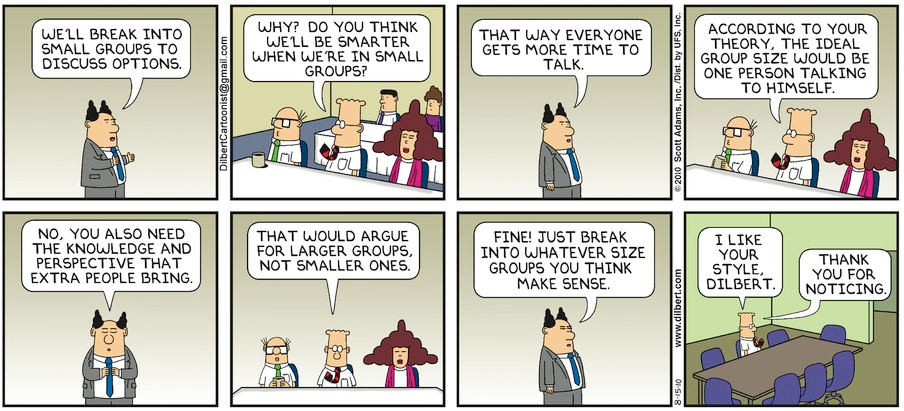
\includegraphics[height=2.85in]{disrupt1.png}
% see http://www.amureprints.com/reprints/classroom
\par \itshape \footnotesize
Dilbert by Scott Adams.
\copyright\ Andrews McMeel Syndication.
\url{http://dilbert.com/strip/2010-08-15}
\end{center}
